\chapter{Technical Formulation}\label{ch:hg-formulation}
\todo{copy the rest of the stuff over here}

\section{Predicates}
\emph{Predicates}\index{state!predicate} are assertions on state.
A predicate~$P$\nomenclature{$P$}{A state predicate}
consists of a set of \emph{clauses}\index{state!predicate!clause}.
$P$ holds in state~$s$%
\nomenclature{$s$}{A concrete state \todo{give better clarification for this elative to the Hoare Graphs; gets introduced earlier though so maybe not?}}
($s\gls{holds}P$) if and only if all clauses hold.

\todo{maybe put more here? Connect to logical predicates}

Breaking it down further, a clause consists of two symbolic expressions\index{symbolic!expression}
and their relation.
A symbolic expression of type \gls{expression} consists of the some combination of the following:
\begin{itemize}
  \item register references (\gls{register}),
  \item flag references (\gls{flag}),
  \item 64-bit words (\gls{word}),
  \item symbolic values (\gls{val}),
  \item memory regions (modeled by an expression for the address and a natural number\index{number!natural} for the size)%TODO: \gls!
  \index{memory!region}, and
  \item the application of an operator\index{symbolic!operator}
  to a list of expressions.
\end{itemize}
In formal notation, this is:
\begin{equation}
  \gls{expression}\coloneqq
  \gls{register}\mid
  \gls{flag}\mid
  \gls{word}\mid
  \gls{val}\mid
  \gls{expression}\times\gls{nat}\mid
  \mathsf{Op}\times[\gls{expression}]
\end{equation}
\nomenclature[operator]{$\coloneqq$}{Indicates that the \ac{rhs} defines the \ac{lhs} for \ac{hg} and \ac{eicfg} work}%
We identify a subset of these symbolic expressions called \emph{constant expressions} (\gls{constant}).
These expressions cannot contain state parts\index{state!part}
such as registers, flags, or memory regions.%
\index{symbolic!register}%
\index{symbolic!flag}%
\index{memory!region}
They represent constants or computations constructed using initial values.%
\index{initial!value}
For example, $\rdio$ denotes the initial symbolic value%
\index{symbolic!value}%
of register~$\reg{rdi}$.
% TODO: This should probably be nomenclature somehow but I'm not sure how
This value does not change during symbolic execution\index{symbolic!execution}.

In notation, clauses\index{state!predicate!clause}
take the form $\gls{expression} \mathbin{\square} \gls{constant}$,%
\nomenclature[operator]{$\square$}{A placeholder for some binary relation}%
\nomenclature[operator]{$\in$}{Indicates that the \ac{lhs} is an element of the set on the \ac{rhs}}
where $\square\in\{=,\neq,<,<_s,\ge,\ge_s\}$.
The~$\square_s$ relations treat their operands as signed,
while the corresponding non-subscripted versions treat their operands as unsigned.

There are also two special clauseless predicates,~\gls{top}%
and~\gls{bot}.
Those special predicates respectively indicate always true (holds for any state) and always false (holds for no state).
\Gls{bot} is also used to indicate an unknown~\gls{constant}.%
\begin{definition}\label{def:join}
  The aforementioned join\index{lattice!join}
  of two predicates~$P$ and~$Q$,%
  \index{state!predicate}
  notation $P\gls{join}Q$,
  is performed by doing a form of range abstraction for symbolic bit-vector values \autocite{rugina2000symbolic}.\index{symbolic!bit vector}
  This is defined as:
  \begin{align*} % \gls{defeq} doesn't seem right here since we already have \gls{equiv}; also don't we have \coloneqq already anyway? Good to be consistent though.
    P\gls{join}Q &\gls{defeq} \bigcup\{\merge(p,q) \mid \langle p,q\rangle\in P\times Q\} \\
    \merge(l=r_1,l=r_2) &\gls{defeq} \{l\ge\min(r_1,r_2),l\le\max(r_1,r_2)\} \\
    \merge(l<r_1,l<r_2) &\gls{defeq} \{l<\max(r_1,r_2)\} \\
    &\vdots\\
    \merge(a,b) &\gls{defeq}
    \begin{cases}
      \{a\} & \text{if }a=b \\
      \varnothing & \text{otherwise}
    \end{cases}
  \end{align*}
\end{definition}
The operator presented in \cref{def:join}
performs a \emph{merge} for each clause pair\index{state!predicate!clause}
$\langle p,q\rangle$
in the Cartesian product\index{Cartesian product} % change to Cartesian!product if you use more references to Cartesian stuff
of its argument predicates.
This merge produces a potentially empty set of clauses
generated from the two clauses supplied to it.
% The union of all sets produced is then taken, resulting in the joined predicate.
While only merge rules for $=$ and $<$ are shown, there are also rules
for the other possible clause operations.
The~$\max$ and~$\min$ functions used are partial;%
\index{function!maximum}%
\index{function!minimum}%
\index{function!partial}
they do not have a result if the maximum/minimum of the expressions supplied to them cannot be determined.%
\index{maximum}
\index{minimum}
This can happen if those symbolic expressions\index{symbolic!expression}
contain unrestricted values\index{symbolic!value}.
In such cases, no clause is produced.
%The supremum, repeated join over a set of predicates, is denoted by $\bigsqcup\square$. % do we even have a supremum here anymore?

\begin{example}
  Let $P=\{a=3,a<\rdio\}$ and $Q=\{a=4,a<\rsio\}$.
  As both predicates\index{state!predicate}
  have equality clauses\index{state!predicate!clause}
  for~$a$, those clauses are merged to produce a pair of clauses denoting that the value of~$a$ lies in the range $[3,4]$.
  Since no maximum can be established between $\rdio$ and $\rsio$, these clauses are dropped.
  Thus, $P\gls{join}Q=\{a\ge 3,a\le4\}$.
\end{example}

As required for a lattice,\index{lattice}
the join\index{lattice!join}
is associative,\index{associative}
commutative,\index{commutative}
and idempotent.\index{idempotent}
Associativity is derived from the fact that set union\index{set!union}
and minimum/maximum%
\index{minimum}%
\index{maximum}
are associative operations.
The join is commutative and idempotent due to the commutativity and idempotency of the merge function. Finally, we have the following for any state~$s$\index{state}:
\begin{lemma}\label{lem:pred_soundness}
  $s\gls{holds}P\vee Q\implies s\gls{holds}P\gls{join}Q$
\end{lemma}
\begin{proof}
  The proof of this lemma consists of two cases:
  \begin{align*}
    s\gls{holds}P &\implies s\gls{holds}P\gls{join}Q \\
    s\gls{holds}Q &\implies s\gls{holds}P\gls{join}Q
  \end{align*}
  Only one of those cases needs to be proven;
  the other follows from the symmetry of the join\index{lattice!join} operation.
  Assuming~$s\gls{holds}P$, we now show $s\gls{holds}P\gls{join}Q$.
  For $s\gls{holds}P\gls{join}Q$ to be true, all of its clauses%
  \index{state!predicate!clause}
  must hold.
  Let~$c$ be one of the clauses resulting from the join.
  It is the result of one of the merge rules.
  Consider the first case, for equality.
  Since $l=r_1$ is a clause in~$P$, we have $l\ge\min(r_1,r_2)$ and $l\le\max(r_1,r_2)$.
  The other cases are similar.

  \todo{double-check this}
\end{proof}

\section{Memory Models}\label{sec:memory-models}
Program analysis\index{program!analysis}
in programs with pointers\index{pointer}
requires efficient alias identification and classification.
When different variables\index{variable}
(or in our case, state parts)\index{state!part}
point to the same memory region, those variables are \emph{aliased}.\index{memory!aliasing}
This is an important issue that must be dealt with for proper predicate transformation.
That is because alias information directs assignments to memory\index{memory!write}.
Specifically, when two state parts are aliased,%
\footnote{Or rather, the symbolic expressions\index{symbolic!expression}
  recorded as being stored in them alias.}
writing to the symbolic location (memory region) specified by one of them will change the value that is read from the symbolic location (memory region) specified by the other.
Unfortunately, it is not always possible to determine whether or not
two state parts alias.

We thus keep track of memory regions read and written during a sequence of execution in structured \emph{memory models}.%
\index{memory!read}%
\index{memory!model}
These memory models store \emph{aliasing}, \emph{separation},%
\index{memory!separation}
and \emph{enclosure}\index{memory!enclosure}
relations for memory regions.\index{memory!region}
This allows for efficient checks of those relations.
Furthermore, constructing them in a nondeterministic\index{nondeterminism}
fashion allows for dealing with multiple potential combinations of relations
between read and written regions in memory.
They are defined by the following data structures:
\begin{align*}
  \gls{memtree} &\coloneqq
  \{\gls{constant}\times\gls{nat}\}\times\gls{mem}
  &
  \gls{mem} &\coloneqq \{\gls{memtree}\}
\end{align*}
That is,
a memory model consists of a possibly empty \emph{forest} of memory trees.%
\index{memory!tree}%
\index{memory!forest}
Each memory tree has as a top-level node,\index{memory!node}
a set of memory regions,\index{memory!region}
and a possibly empty sub-forest that holds its child regions.
Two regions in the same node set alias.
The child regions are enclosed in their parents.
Finally, regions in sibling nodes are separate.

\begin{example}
  Consider the two memory models presented in \cref{fig:mem}.
  These memory models involve three regions: $\region{\rdio}{8}$,
  $\region{\rsio}{8}$ and $\region{\rsio+4}{4}$.
  The memory models depict the case where $\rdio$ and $\rsio$ alias and not alias.
  As stated above, sibling nodes on the same level are separate, while children are enclosed by their parents.
  Regions within the same node alias.
  Thus, \cref{fig:memA} shows a situation with
  two top-level regions aliasing and the child region they share.
  \Cref{fig:memB}, meanwhile, shows a situation where the two top-level regions do not alias,
  and thus only one of those regions contains an enclosed child.
\end{example}
\begin{figure}
  \hspace*\fill
  \subcaptionbox{Aliasing\label{fig:memA}}{
    \begin{tikzpicture}[every node/.style=draw]
      \node (a) {$\{\region{\rdio}{8},\region{\rsio}{8}\}$};
      \node[below=of a] (b) {$\region{\rsio+4}{4}$};

      \draw[->] (a) -- node [draw=none,midway, left, fill=white] {\rotatebox{90}{\gls{enclosed}}}(b); % keeping spacing aligned
    \end{tikzpicture}%
  }
  \hfill
  \subcaptionbox{No aliasing\label{fig:memB}}{%
    \begin{tikzpicture}[every node/.style=draw]
      \node (a) {$\region{\rdio}{8}$};
      \node[right=of a] (b) {$\region{\rsio}{8}$};
      \node[below=of b] (c) {$\region{\rsio+4}{4}$};

      \draw (a) -- node [draw=none,midway, above, fill=white] {\gls{separate}} (b) ;
      \draw[->] (b) -- node [draw=none,midway, left, fill=white] {\rotatebox{90}{\gls{enclosed}}} (c);
    \end{tikzpicture}%
  }
  \hspace*\fill
  \caption{Memory model examples}
  \label{fig:mem}
\end{figure}

\begin{definition}\label{def:memory-relations}
  Let~$s$ be a concrete state and let $r_0=\region{e_0}{n_0}$ and $r_1=\region{e_1}{n_1}$ be two regions in memory.
  Then, the properties of \emph{aliasing}, \emph{separation}, and \emph{enclosure}, notations \gls{alias}, \gls{separate}, and \gls{enclosed}, respectively, are defined as:
  \begin{align*}
    r_0\gls{alias}r_1 &\gls{defeq}s \gls{holds} e_0 = e_1 \wedge n_0 = n_1 \\
    r_0\gls{separate}r_1 &\gls{defeq}s \gls{holds} (e_0 + n_0 \le e_1) \vee (e_1 + n_1 \le e_0)\\
    r_0\gls{enclosed}r_1 &\gls{defeq}s \gls{holds} e_0 \ge e_1 \wedge e_0 + n_0 \le e_1 + n_1
  \end{align*}
\end{definition}
Such relations hold \emph{necessarily} if and only if they hold in all concrete states~$s$.
For example, $\region{\rsio}{4}\gls{separate}\region{\rsio+4}{4}$ is a necessarily-separate relation as there are no values of~$\rsio$ for which those two regions are not separate.
The \ac{smt} solver/theorem prover Z3 \autocite{de2008z3} is used to establish whether these ``necessarily''-relations hold for symbolic addresses\index{symbolic!address}
given the current state predicate\index{state!predicate}.
This is done via expression translation directly to Z3's bit-vector\index{numeric!bit vector}
representations, meaning no information is lost in the conversion
and when querying the constructed logical formulas.

In our Z3 interface, each operation to determine aliasing/separation/enclosure
also takes a predicate as an additional argument.
This is used to provide additional assumptions for necessarily-calculations,
as in isolation it is often not possible to determine the relationships between
entirely symbolic expressions\index{symbolic!expression}
that do not share symbolic values.\index{symbolic!value}
While the predicate may not help in all cases,
there may be instances where a relation between two symbolic values
or expressions was expressed previously in the program.

We further extend the notation in \cref{def:memory-relations} to memory trees.
That is, $t_0\gls{separate}t_1$ denotes that all regions in~$t_0$ are necessarily separate from all regions in~$t_1$.
Notation $t_0\gls{alias}t_1$ ($t_0\gls{enclosed}t_1$) denotes that some region in the top node of~$t_0$ and some region in the top node of~$t_1$ necessarily alias (are enclosed).
%Similarly,  denotes that some region in the top node of~$t_0$ is necessarily enclosed in some region of the top node of~$t_1$.

\subsection{Insertion}
Construction of a memory model is performed
using the recursive \gls{insertM} function shown below.
It takes as input a memory tree~$t$ and the current memory model~$M$.
The current predicate~$P$ is also supplied
to assist in the region relationship analysis.
However, it is elided from the below presentation as it is a read-only value
that is passed along through the function call chain.
For output, function \gls{insertM} produces, nondeterministically,
a set of new memory models based on all possible pointer relationships
for the newly-inserted region.
If no necessarily-relation can be established between~$t$ and any tree in~$M$, then all trees possibly overlapping with~$t$ are destroyed (see \cref{something-from-the-intro}).
If a necessarily-relation can be established between tree~$t$ and some tree already in~$M$, then only the relevant memory models need to be produced.

To ensure that the invariants for the memory model~$M$ being inserted into
are not violated, the external interface to the function takes a single region,~$r$, instead of a memory tree.
This region is embedded in a minimal memory tree,
$\langle \{r\},\varnothing\rangle$,
which is then supplied to the below function.

\begin{definition}[Memory Tree Insertion]\label{def:insert}
  Let $t_0 = \langle R_0,M_0\rangle$ and $t_1 = \langle R_1,M_1\rangle$ be two trees. Function
  \gls{insertM} of type $\gls{memtree}\times\gls{mem}\times\gls{predicate}\rightarrow\{\gls{mem}\}$
  is defined as follows:
  \begin{align*}
    (t_0,\varnothing) &\gls{defeq} \{t_0\}\notag \\
    \gls{insertM}[(t_0,t_1\cons M)] &\gls{defeq} \begin{cases}
      \gls{insertM}[_\text{AL}(t_0,t_1,M)] & \text{ if } t_0\gls{alias}t_1 \\
      \gls{insertM}[_\text{SEP}(t_0,t_1,M)] & \text{ if } t_0\gls{separate}t_1 \\
      \gls{insertM}[_\text{ENC}(t_0,t_1,M)] & \text{ if } t_0\gls{enclosed}t_1 \\
      \gls{insertM}[_\text{CON}(t_0,t_1,M)] & \text{ if } t_1\gls{enclosed}t_0 \\
      \mbox{destroy}(t_0, M)  & \text{otherwise}
    \end{cases}
  \end{align*}
  \todo{fix the formatting! though switching to equation* already got me halfway thebre}
  Notation $a \cons X$ denotes $\{a\} \cup X$ \todo{put this in glossary}.
  \begin{equation*}
    \begin{array}{lcl}
      \gls{insertM}_\text{AL}(t_0,t_1,M) &\gls{defeq}& \\
      \multicolumn{3}{r}{\{(R_0\cup R_1, M') \cons M \mid M' \in \mathsf{fold}(\gls{insertM}, M_0 \cup M_1) \}} \\
      \gls{insertM}_\text{SEP}(t_0,t_1,M) &\gls{defeq}& \{t_1\cons M'\mid M'\in\gls{insertM}[(t_0,M)]\} \\
      \gls{insertM}_\text{ENC}(t_0,t_1,M) &\gls{defeq}& \{\langle R_1,M'\rangle\cons M\mid M'\in\gls{insertM}[(t_0,M_1)]\} \\
      \gls{insertM}_\text{CON}(t_0,t_1,M) &\gls{defeq}& \\
      \multicolumn{3}{r}{ \{\gls{insertM}[(t',M)]\mid t'\in\{\langle R_0,M'\rangle\mid M'\in \gls{insertM}[(t_1,M_0)]\}\}}
    \end{array}
  \end{equation*}
\end{definition}
As further explanation, let $t_0 = \langle R_0,M_0\rangle$ be the tree to be inserted and $t_1 = \langle R_1,M_1\rangle$ be a tree already in the memory model.
\begin{enumerate}
  \item If~$t_0$ and~$t_1$ alias, then they are combined by taking the union of their nodes.
  Their child regions are not necessarily the same, however.
  Thus, subtrees are then reinserted using a $\mathsf{fold}$ \todo{change up this notation/styling}.
  \item If trees~$t_0$ and~$t_1$ are separate, then tree~$t_0$ is recursively inserted into the remainder of the memory model and~$t_1$ is added without modification.
  \item If~$t_0$ is enclosed in~$t_1$, it is recursively inserted into the sub-forest of~$t_1$.
  Each memory model~$M'$ thus obtained is wrapped in a tree $\langle R_1,M'\rangle$.
  The remainder of memory model~$M$ is unmodified.
  \item Finally, if $t_1$ is enclosed in $t_0$, then $t_1$ is recursively inserted into the sub-forest of $t_0$.
  Each memory model~$M'$ thus obtained is wrapped in a tree $t'=\langle R_0,M'\rangle$.
  That tree is then recursively inserted into memory model~$M$.
\end{enumerate}
\begin{example}\label{ex:example_snippet}
  Consider the three-instruction assembly snippet below.
  This snippet first stores the value \num{1000} in the eight-byte memory region
  pointed to by \rsi, then stores the value \num{1001}
  in the four-byte region pointed to by $\rsi+4$.
  Finally, it stores the value \num{1002} in the eight-byte region
  pointed to be \rsi.
  If the current state allows aliasing and separation between $\region\rdi8$ and $\region\rsi8$, then
  these three instructions will result in the two memory models in \cref{fig:mem}.
  Note that region $\region{\rsi+4}4$ is necessarily enclosed in region $\region\rsi8$.
  \begin{lstlisting}[style=x64]
    mov qword ptr [rdi],   1000
    mov dword ptr [rsi+4], 1001
    mov qword ptr [rsi],   1002
  \end{lstlisting}
\end{example}
A memory model~$M$ \emph{holds} in concrete state~$s$ if all siblings are separate and all trees hold.
A tree holds if its node contains only aliasing regions and all trees in its sub-forest are enclosed. Formally, this is expressed as:
\begin{definition}
  A memory model~$M$ \emph{holds} in state~$s$, notation $s\gls{holds}M$,
  if and only if:
  \begin{equation*}
    (\forall t_0, t_1\in M\sepdot t_0\neq t_1\implies s\gls{holds}t_0 \gls{separate}t_1) \wedge (\forall t\in M\sepdot s\gls{holds}t)
  \end{equation*}
  A memory tree~$t = \langle R,M\rangle$ \emph{holds} in state~$s$, notation $s\gls{holds}t$, if and only if:
  \begin{equation*}
    (\forall r_0,r_1 \in R\sepdot s\gls{holds}r_0\gls{alias}r_1) \wedge (\forall t'\in M\sepdot s\gls{holds}t'\gls{enclosed}t) \wedge (s\gls{holds}M)
  \end{equation*}
\end{definition}
\begin{example}
  Consider again the memory models in \cref{fig:mem}
  for the assembly snippet in \cref{ex:example_snippet}.
  The aliasing memory model in \cref{fig:memA}
  holds only in states where $\rdio=\rsio$.
  Meanwhile, the non-aliasing memory model in \cref{fig:memB}
  holds only in states where $\rdio+8\le\rsio$ or $\rsio+8\le\rdio$.
\end{example}

\todo{I changed up the wording but this still seems a bit abrupt, not sure how best to lead into the completeness discussion}
An important quality our insertion function must possess is \emph{completeness}.%
\index{completeness}
That is, the produced memory models should cover any possible relation between inserted region~$r$ and any region~$r'$ already present in the memory model.
To formulate completeness, we use~$R(M)$ to denote the set of regions in memory model~$M$ and $\mathcal{R}(M)$ to denote the set of relations.
\todo{I still want to revise this into my own words and notation if possible}
For example, we have $(\region\rdio8\gls{alias}\region\rsio8) \in \mathcal{R}(M)$ for the memory model in \cref{fig:memA}.

\todo{This lemma and proof are the most important things to put in my own words}
\begin{lemma}\label{lem:insert}
  Let~$r_0$ and~$M$ be a region and a memory model, respectively.
  Also let~$f$ of type $\gls{constant}\times\gls{nat}\mapsto \{ \gls{alias},  \gls{separate}, \gls{enclosed},\gls{encloses}\}$ be some mapping that provides a relation between~$r_0$ and~$r'$ for any region~$r'$ currently in memory model~$M$.
  Assume that $f$ is possibly true:
  \todo{glossary entry for $\models$}
  \begin{equation*}
    \exists s \sepdot s \gls{holds}M \wedge (\forall r' \in R(M) \sepdot s \models r_0~f(r')~r')
  \end{equation*}
  Then, insertion of region $r_0$ into $M$ will produce at least a corresponding memory model:
  \begin{equation*}
    \exists M' \in \gls{insertM}[(\langle r_0,\varnothing\rangle,M)] \sepdot \{ (r_0~f(r')~r') \mid r' \in R(M) \} \subseteq \mathcal{R}(M')
  \end{equation*}
  In words, there exists some memory model that contains all relations of mapping~$f$.
\end{lemma}
\begin{proof}
  The proof is by induction.
  The base case is trivial.
  For the inductive case, we insert region~$r$ into $\{t_1\} \cup M$.
  Four cases are possible:
  \begin{enumerate}
    \item Region $r_0$ necessarily aliases with $t_1$.
    In this case, since mapping $f$ is possibly true, it must assign \gls{alias} to all top-level regions of $t_1$, \gls{encloses} to all other regions in $t_1$ and \gls{separate} to all regions in $M$.
    The created memory model contains these relations.
    \item Region $r_0$ is necessarily separate from $t_1$.
    In this case, since mapping $f$ is possibly true, it must assign \gls{separate} to any region in $t_1$.
    Thus, tree $t_1$ is not modified and region $r_0$ is recursively inserted into $M$.
    The \ac{ih} then finishes the proof.
    \item Region $r_0$ is necessarily enclosed by a top-level region of $t_1$.
    Since mapping $f$ is possibly true, it must assign \gls{separate} to all regions of $M$.
    Therefore, the insertion function does not modify $M$.
    Since $r_0$ and $r_1$ do not alias, the top-level regions $R_1$ of tree $t_1$ can remain unmodified as well.
    Region $r_0$ is recursively inserted into a child of $t_1$, proof follows from the \ac{ih}.
    \item Tree $r_1$ is necessarily enclosed into region $r_0$.
    In this case, since mapping $f$ is possibly true, it must assign $\succeq$ to all regions of $t_1$.
    Therefore, tree $t_1$ is recursively inserted as subtree of $r_0$, producing a set of trees.
    For the remaining regions not in $t_1$, $f$ can hold arbitrary relations.
    Therefore any $t'$ in the produced set is recursively inserted into $M$.
    Again, the \ac{ih} then finishes the proof.
    \item As an extra case, consider when no relation can necessarily be established. In that case, all of the above proofs apply, as memory models are generated for each possible case. \todo{Shouldn't I include this part? Not sure why it was commented out.}
  \end{enumerate}
\end{proof}

\subsection{Joining}
As with state predicates, memory models have a join operation.
\begin{definition}\label{def:mem-join}
  The join of two memory models~$M_0$ and~$M_1$,
  notation $M_0\gls{join}M_1$, is recursively defined as:
  \begin{align*}
    M_0\gls{join}M_1 &\gls{defeq} \left\{\gls{join}(T) \relmiddle| T\in\faktor{M_0 \cup M_1}{\gls{comparable}[^+]}\right\}\notag \\
    \langle R_0,.\rangle\gls{comparable}\langle R_1,.\rangle &\gls{defeq} R_0 \cap R_1\neq\varnothing\notag \\
    \gls{join}(T) &\gls{defeq} \left\langle\bigcap\{R\mid\langle R,.\rangle\in T\}, \bigsqcup\{M\mid\langle.,M\rangle\in T\}\right\rangle
  \end{align*}
\end{definition}
This operation partitions the memory trees in $M_0$ and $M_1$ based on
equivalence relation $\gls{comparable}[^+]$.
This equivalence relation is the transitive closure
of relation \gls{comparable}, which determines if
its two memory trees have any top-level regions in common.
In other words,
all memory trees that have one or more top-level regions in common are put in an equivalence class and are thus joinable.
The operator \gls{join} then performs the join operation
for each equivalence class of memory trees,
taking the intersection of all their region sets
and the supremum of their child memory models.
\begin{example}
  Consider two memory models~$M_0$ and~$M_1$ where both have the top node $\region\rdio8$.
  We add the distinction that~$M_0$ has an enclosed child $\region\rdio4$ and~$M_1$ has an enclosed child $\region{\rdio+4}4$. The result of joining~$M_0$ and~$M_1$ is a single memory model with $\region\rdio8$ as its top node and the two child regions in separate sibling nodes.
\end{example}

\begin{figure}
  \hspace*\fill
  \subcaptionbox{Alternate memory model\label{fig:otherMem}}{
    \hspace{3ex}
    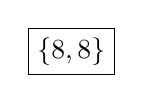
\begin{tikzpicture}[>=stealth, every node/.style={draw}]
      \node (a) {$\{\region\rdio8,\region\rdxo8\}$};
    \end{tikzpicture}%
    \hspace{3ex}
  }
  \hfill
  \subcaptionbox{Join result\label{fig:otherMemJoin}}{
    \hspace{2ex}
    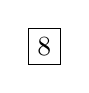
\begin{tikzpicture}[>=stealth, every node/.style={draw}]
      \node (a) {$\region\rdio8$};
    \end{tikzpicture}%
    \hspace{2ex}
  }
  \hspace*\fill
  \caption{Join with alternate memory model}\label{fig:otherJoin}
  %\Description{This shows an alternate memory model (on the left,
    %containing two eight-byte regions with separate symbolic variable bases)
    %that is joined with the memory model from Figure~\ref{fig:memA}
    %(where one of the top-level regions is shared),
    %resulting in the memory model shown on the right in the figure.
    %(only that shared top-level region is present)}
\end{figure}
\begin{example}
  First, consider the memory models shown in \cref{fig:mem}.
  Since the top nodes share a region, the two trees belong to the same equivalence class.
  The intersection of all of the region alias sets is:
  \begin{equation*}
    \{\region\rdio8,\region\rsio8\}\cap
    \{\region\rdio8\}\cap\{\region\rsio8\}.
  \end{equation*}
  As this intersection produces~$\varnothing$,
  the result of the join is~$\varnothing$, an empty memory model.
  Second, consider the join of the memory model shown in \cref{fig:memA}
  with the one shown in \cref{fig:otherMem}.
  The result of that join is the memory model shown in \cref{fig:otherMemJoin}.
  This is because all top-level memory trees involved in the merge share
  a region, $\region\rdio8$, but have no comparable children.
\end{example}

To strengthen our arguments, we prove that the join over memory models we have provided is sound.
\begin{lemma}\label{lem:mem_soundness}
  Let~$s$ be a state and~$M_0$ and~$M_1$ be memory models. Then:
  \begin{equation*}
    (s\models M_0 \vee M_1) \implies (s\models M_0\gls{join}M_1)
  \end{equation*}
\end{lemma}
\begin{proof}
  \todo{will look through this proof again for more my terms}
  Let $r_0\mathbin{\square}r_1$ be a relation in $\mathcal{R}(M_0\gls{join}M_1)$.
  If $\square$ is \gls{alias}, then both regions $r_0$ and $r_1$ must have been present in all trees in the corresponding equivalence class.
  The relation thus held in either $M_0$ or $M_1$.
  If $\square$ is \gls{separate}, then the two regions are from trees generated from different equivalence classes. Since they are from trees that do not share a top-level region, the original trees in either $M_0$ or $M_1$ are separate as well.
  Similar reasoning applies for the other cases.
\end{proof}

\begin{definition}
  \todo{did we introduce the \emph{symbolic} state terminology before this?}
  The join of two symbolic states $\sigma_0=\langle P_0,M_0\rangle$
  and $\sigma_1=\langle P_1,M_1\rangle$, notation $\sigma_0\gls{join}\sigma_1$, is:
  \begin{equation*}
    \sigma_0\gls{join}\sigma_1\gls{defeq}\langle P_0\gls{join}P_1,M_0\gls{join}M_1\rangle
  \end{equation*}
\end{definition}

Do keep in mind that this join in its full form \emph{loses} information.
It can thus only be applied in a sound fashion for postcondition weakening \autocite{hoare1969axiomatic}.
In other words, dropping clauses and performing state cleanup
serve only to reduce state constraints; they never add additional ones.
In practice, this loss of information means that we may produce a state
that would not actually be encountered during program execution.
Alternatively, we may be unable to resolve some indirections or prove some return addresses, which would result in additional annotations generated or even tool failure.
Despite this, in cases with successful completion and no annotations produced,
we will always produce all states that would be encountered during concrete execution.

\section{Algorithm}\label{sec:algorithm}
\Cref{alg:invgen} provides the base functionality for \ac{hg} extraction.
That base functionality is then extended in two ways:
\begin{enumerate}
  \item the addition of a context-free approach to function calls (see \cref{subsec:function_calls}) and
  \item the prevention of states from being joined when they are incompatible (i.e.\ not matching \cref{def:compatibility}). \todo{index entry that just points to compatible's?}
\end{enumerate}
In order to do this, the algorithm maintains two objects.
First, a \gls{bag} of the produced symbolic states that have yet to be explored.
Function \gls{explore} is repeatedly called until that \gls{bag} is empty.
Second, the current \ac{hg} \gls{hg}.
When the \gls{bag} is empty, \gls{hg} is the final \ac{hg}.

Furthermore, the algorithm requires a function~\gls{step-hg-semantics} that models instruction semantics.
Our implementation supports a wide range of \gls{arch} instructions,
including (conditional) moves and jumps as well as
arithmetic, logical and bit-vector operations (sufficient to deal with all Xen binaries).\todo{glossary for Xen}
Given a supported instruction and a suitable memory model,
function~\gls{step-hg-semantics} transforms its supplied predicate
into a set of predicates \todo{glossary entry for lots of these terms would be nice}
by symbolically executing the single instruction.
The memory model allows~\gls{step-hg-semantics} to take into account information on pointer relations
when performing symbolic execution using destination operands
that reference memory locations.


The algorithm also requires an expression evaluation function
$\gls{eval}:\gls{expression}\times\gls{pred}\mapsto\gls{constant}$,
which maps an expression (containing registers, flags, and dereferenced memory regions)
to a constant expression.
To that end, it requires the predicate of the current symbolic state.
No memory model information is required for this evaluation;
that information is only required when writing to a location in memory.
\begin{definition}\label{def:eval}
  Given predicate $P$, \todo{glossary entry for the variable?} the evaluation of an expression $e$ is defined as follows:
  \begin{equation*}
    \gls{eval}(e,P)=\begin{cases}
      v & \text{if $e = v$ is a clause in }P \\
      \gls{bot} & \text{otherwise}
    \end{cases}
  \end{equation*}
\end{definition}

That evaluation function is then used by the algorithm in the process of executing steps according to the following step function:
\begin{definition}
  The \emph{symbolic state step function} for symbolic state $\sigma = \langle P,M\rangle$, notation $\gls{step-hg}[(\sigma)]$, is defined as:
  \begin{equation*}
    \begin{array}{l}
      ~~\gls{step-hg}[(\sigma)]\gls{defeq}\{ \langle P',M'\rangle \mid P' \in \gls{step-hg-semantics}[(P,M')] \wedge M' \in \gls{insertM}[(R,M)] \} \\
      \mbox{\normalfont{\textbf{where}}}\\
      ~~\begin{aligned}
        R &\gls{defeq} \{ [\gls{eval}[(a,P)],s] \mid [a,s]\text { used by instruction } i \} - \{\gls{bot}\}\\
        i &\gls{defeq} \gls{fetch}(\gls{eval}[(\rip, P)])
      \end{aligned}
    \end{array}
  \end{equation*}
\end{definition}
Given the current symbolic state $\sigma$, the set of next symbolic states is obtained by performing the following two actions:
\begin{itemize}
  \item inserting relevant regions into the current memory model and
  \item applying predicate transformation to the current predicate.
\end{itemize}
The set of regions is obtained by investigating the operands of the current instruction.
\begin{example}[Regions from Instructions]
  The instruction \inlineasm{mov qword ptr [rax + 4*rdi], rax} results in one region, $\region{\rax + 4*\rdi}8$.
\end{example}
That region is---given the current predicate---evaluated to a constant.
\begin{example}[Evaluation of Region Part]
  If the current predicate contains $\rax=\mathtt{0x100}$ and $\rdi=\rsio$, then evaluation of $\rax + 4*\rdi$ produces the constant $0x100 + 4*\rsio$.
\end{example}
If the current predicate does not contain enough information to evaluate a state-part-containing region to a constant region,
evaluation for that region produces~\gls{bot} and the region is not inserted.
Otherwise, the successfully-evaluated region is inserted.
The latter case overapproximates any relation (e.g., aliasing, separation) the new region may have with the current memory model.

It is also possible for lack of information to result in inability to continue predicate execution.
Specifically, if no bounded set of continuation states can be determined,
we produce an annotation and stop further exploration from that state.
This primarily occurs for unresolved indirect jumps and calls.

\begin{definition}[Compatibility]\label{def:compatibility}
  Two symbolic states $\sigma$ and $\sigma'$ are \emph{compatible}, notation $\sigma_0\gls{compatible}\sigma_1$, if and only if their instruction pointers ($\rip$) are equal.
  States will only be joined when they are compatible.
\end{definition}
An extension to the base algorithm presented below in \cref{alg:invgen} modifies this definition.
Specifically, it adds the constraint that states are not considered compatible when shared registers are assigned different immediate values that directly influence control flow
(for example, when the immediates are loaded from a jump table).
In general, it is impossible to know whether or not a stored value will influence future control flow.
However, it is sufficient to detect situations in which values will \emph{likely} influence future control flow.

This modification to compatibility does not cause any soundness issues.
If a value was erroneously deemed to influence future control flow, then we have unnecessarily explored paths that could have been joined earlier, but this only affects analysis time and not soundness.
\todo{reference join by textual form somehow?}
Joining states that contain immediate values that turn out to be necessary to assess future control flow is no issue either.
It will merely lead to unresolved indirections or errors being reported by the analysis, and soundness will still not be affected.

Concretely, if two states have assignments of different immediate pointers to instructions%
\footnote{Concrete pointer values that fall within the range of the text section of the binary}
to the same state part, then we do not join those pointers to an abstract value.
Instead, we continue exploration from both states.
This is because those immediate values are highly likely to influence future control flow.
Such an approach causes less abstraction, but does allow us to resolve more indirections.
In very specific cases it even results in more preciseness.

\subsection{Base Algorithm}

\begin{algorithm}
  \caption{Base Version of Hoare Graph Extraction}
  \label{alg:invgen}
  \algnewcommand{\IIf}[2]{\State\algorithmicif\ #1\ \algorithmicthen~#2}
  \begin{algorithmic}[1]
    \Function{explore}{} \todo{gls link for {explore} here?}
      \State pop $\sigma$ from \gls{bag}\label{line:pop}
      \If{$\exists \sigma_c \in\gls{hg}\sepdot \sigma_c\gls{compatible}\sigma$}\label{line:compat}
        \IIf{$\sigma \sqsubseteq \sigma_c$}{\Return}\label{line:terminate}
        \State $\sigma_j \coloneqq \sigma\gls{join}\sigma_c$\label{line:join}
        \State $\gls{hg}[\sigma_c \coloneqq \sigma_j]$
      \Else
        \State $\sigma_j \coloneqq \sigma$\label{line:nocompat}
      \EndIf
      \ForAll{$\sigma' \in \gls{step-hg}[(\sigma_j)]$}\label{line:forall}
        \State $\gls{hg} ~\gls{pluseq}~ (\sigma_j, \sigma')$
        \If {$\gls{eval}(\rip, \gls{pred}[(\sigma')])$ is not immediate}
          \State \textbf{annotate, stop further exploration}\label{line:undsound}
        \Else
          \State $\gls{bag}\gls{pluseq}\sigma'$\label{line:addbag}
        \EndIf
      \EndFor\label{line:endforall}
    \EndFunction
  \end{algorithmic}
\end{algorithm}

Let $\sigma$ be some symbolic state from the~\gls{bag} (\cref{line:pop}).
Function \gls{explore} first searches for a current symbolic state~$\sigma_c$ already in the current~\gls{hg} that is compatible (\cref{line:compat}).
If such a state exists and it is more abstract (based on ordering $\sqsubseteq$)
\todo{glossary entry for this ordering, and also probably needs to be explained earlier or in the background chapter section on lattices!}
than state~$\sigma$, no further exploration is necessary (\cref{line:terminate}).
Otherwise,~$\sigma$ and~$\sigma_c$ are joined (\cref{line:join}).
The~\gls{hg} is modified by replacing the current state with the joined one.
This replacement maintains all current edges: only the state is modified.
Symbolic state~$\sigma_j$ is the state to be explored further.
If no compatible state exists in the current~\gls{hg}, then~$\sigma$ is the state to be explored further (\cref{line:nocompat}).
Exploration occurs at \crefrange{line:forall}{line:endforall}.
For every successor~$\sigma'$ (possibly none), an edge is added to the~\gls{hg}.
If, for some successor evaluation of the instruction pointer,~$\rip$ does not produce an immediate concrete value, there are two possibilities.
Either
\begin{enumerate}
  \item a return statement has been encountered (after which \rip\ is set to the symbol pushed to the top of the stack in the initial state), or
  \item the current symbolic state does not provide sufficient information to resolve the computation of \rip\ (because of an indirect branch, for example).
\end{enumerate}
In the second case, the state is annotated with an unsoundness warning (\cref{line:undsound}) and the algorithm terminates early.
Otherwise, the successor is added to the bag.

\paragraph{Soundness}
\todo{Another relation to glossarify}
To formulate soundness and present a proof, we first define a relation $\mathbf{R}$
\todo{this relation needs a glossary entry!}
between the concrete transition system and the \ac{hg}.
We then prove \cref{lem:simulation}, which shows that this relation is a simulation.
As a direct result of this lemma, any concrete path can be simulated by a path consisting of symbolic steps produced by function~\gls{step-hg}.

\begin{definition}
  A concrete state~$s$ is \emph{related to} symbolic state $\sigma = \langle P,M \rangle$, notation $s~\mathbf{R}~\sigma$, if and only if:
  \begin{equation*}
    s~\mathbf{R}~\sigma \gls{defeq} (s\gls{holds}P) \wedge (s\gls{holds}M)
  \end{equation*}
\end{definition}

\begin{lemma}\label{lem:simulation}
  Assume that predicate transformation~\gls{step-hg-semantics} is correct:
  \begin{equation*}
    \forall s~s' \sepdot s \rightarrow_B s' \wedge (s\gls{holds}P) \implies \exists Q\in\gls{step-hg-semantics}[(P,M)] \sepdot s'\gls{holds}Q.
  \end{equation*}
  Then relation $\mathbf{R}$ is a simulation between the concrete transition system and the transition system obtained by abstract step function \gls{step-hg}:
  \begin{equation*}
    \forall s~s' \sepdot s \rightarrow_B s' \wedge s~\mathbf{R}~\sigma \implies \exists \sigma' \in \gls{step-hg}[(\sigma)] \sepdot s'~\mathbf{R}~\sigma'
  \end{equation*}
\end{lemma}
\begin{proof}
  Let $s$ and $\sigma$ be two related states.
  Hence $(s\gls{holds}P) \wedge (s\gls{holds}M)$.
  By correctness of~\gls{step-hg-semantics}, we obtain a predicate $Q\in\gls{step-hg-semantics}[(P,M)]$ such that $s'\gls{holds}Q$.
  By \cref{lem:insert} (completeness of the insertion function), the memory model that holds in state~$s'$ is generated.
  Since the step function overapproximates by taking any combination of predicates in $\gls{step-hg-semantics}[(P,M)]$ and generated memory models, there exists at least one symbolic state that is related to~$s'$.
\end{proof}

\begin{definition}
  \Ac{hg} $H = \langle \Sigma, \sigma_I, \rightarrow_\Sigma\rangle$ is \emph{sound} with respect to binary $B = \langle a_e, \gls{fetch}, S, \rightarrow_B \rangle$, notation $\gls{sound}(H,B)$, if and only if:
  \begin{equation*}
    \gls{sound}(H,B) \gls{equiv} \forall s_0 \rightarrow_B^\ast s \rightarrow_B s' \sepdot \exists \sigma \rightarrow_\Sigma \sigma' \sepdot s~\mathbf{R}~\sigma \wedge s'~\mathbf{R}~\sigma'
  \end{equation*}
\end{definition}
In words, for every reachable transition from~$s$ to~$s'$ in the binary, there must exist a related transition in the \ac{hg}.

%\subsubsection{Termination}
%\begin{lemma}
%  Algorithm~\ref{alg:invgen} terminates.
%\end{lemma}
%\begin{proof}
%
%\end{proof}
%
%\subsubsection{Pulling it all together}
\begin{theorem}[Soundness]\label{thm:algo_soundness}
  \Cref{alg:invgen} constructs a sound \ac{hg}.
\end{theorem}
\begin{proof}
  The structure of the algorithm is close to \iac{dfs}.
  For that reason, the white-path lemma is used to prove soundness \autocite{cormen2009introduction}.\todo{glossary entry!}
  For a normal \ac{dfs}, the white-path lemma states that the \ac{dfs} will eventually explore some state~$s'$ if and only if there exists some state~$s$ currently in the bag \emph{and} there exists a ``white'' path from~$s$ to~$s'$.
  A key difference between \cref{alg:invgen} and a normal \ac{dfs} is that states are joined.
  For the sake of this proof, a state is therefore considered ``white'' if the current \ac{hg} contains no compatible state that is equal or more abstract (under $\sqsubseteq$).
  We reformulate the white-path lemma as follows:
  \begin{equation*}
    \begin{array}{l}
      \indent\mathsf{sup}(\sigma') \text{ is explored } \Longleftrightarrow \\
      \indent\exists \sigma \in\gls{bag}\sepdot \exists \pi = [\sigma, \dotsc, \sigma'] \sepdot \mathsf{white}(\pi)
      \\
      \textbf{where}
      \\
      \mathsf{sup}(\sigma') \gls{equiv} \bigsqcup \{ \sigma'' \mid \sigma''\gls{compatible}\sigma' \wedge \exists \pi = [\sigma, \dotsc, \sigma''] \sepdot \mathsf{white}(\pi) \}
    \end{array}
  \end{equation*}
  In words, $\mathsf{sup}(\sigma')$, the supremum of all compatible states that are currently reachable through white paths, is explored by the algorithm if and only if there exists a white path from some~$\sigma$ currently in the bag to~$\sigma'$.
  Given this version of the white-path lemma, it directly follows that if the bag initially contains the initial state only:
  \begin{equation*}
    \mathsf{sup}(\sigma') \mbox{~is explored} \Longleftrightarrow \sigma' \mbox{~is reachable from $\sigma_0$}
  \end{equation*}
  Now let~$s$ be a reachable concrete state and $s'$ be a successor.
  \Cref{lem:simulation} shows that the path from~$s_0$ to~$s$ can be simulated by a path of related symbolic states.
  Let~$\sigma$ be the symbolic state related to concrete state~$s$, i.e., $s~\mathbf{R}~\sigma$.
  Since~$\sigma$ is reachable, $\mathsf{sup}(\sigma)$ is explored.
  We thus have
  $s~\mathbf{R}~\sigma \implies s~\mathbf{R}~\mathsf{sup}(\sigma)$.
  This is a direct implication of \cref{lem:mem_soundness}: since joining makes the states more abstract, it makes the set of related concrete states larger.
  \Cref{line:forall} will then explore some state $\sigma' \in \gls{step-hg}[(\sigma_j]$.
  By \cref{lem:simulation}, we have $s'~\mathbf{R}~\sigma'$.
\end{proof}

\subsection{Extension: Function Calls}\label{subsec:function_calls}
The base algorithm as presented in \cref{alg:invgen} does not treat function calls as special instructions.
This is unsatisfactory for two reasons.
First, for \emph{external} function calls, a function~\gls{step-hg-semantics} that transforms the predicate may not be available.
External function calls are dynamically linked and thus the assembly instructions are not available during static analysis.
Second, even though \emph{internal} function calls theoretically pose no problem, simply unfolding every function call prevents scalability.
We present an extension to the algorithm that treats internal function calls compositionally. That is, it ensures that each function is explored only once.

\subsubsection{External Functions}
%An assembly instruction of the form \texttt{call op} is recognized as an external call as soon as the operand can be resolved as an address that belongs to some \texttt{.plt} section.
%This is specific to the ELF format.
%Instead of symbolically executing the instructions found in the \texttt{.plt} section, these instructions are used to derive a function address.
%That address is looked up in the symbol table of the binary.
%If that table associates a name with the address, then that name is the function name of the external function.


The function name is matched against a list of hard-coded function names that are known to be terminating, such as \inlineasm{exit} and \inlineasm{stack_chk_fail}.
In case of a terminating function, function \gls{step-hg} will produce the empty set, stopping further exploration from the current state.
Otherwise, the function is some unknown external function.
We make the assumption that this unknown function adheres to the 64-bit System V \ac{abi}'s calling convention.
Function \gls{step-hg} therefore modifies the current state by assigning~\gls{bot} to all registers, flags and heap regions currently in the state that may not be assumed to be preserved by a function call.
In other words, only the clauses concerning the stack frame and callee-saved non-volatile registers are kept.
Similarly, all relations in the memory model concerning the heap are removed.
We call this \emph{cleaning} the current symbolic state.
As with the join operation, this usage is sound as the end result is always a weakening of the postcondition.

\subsubsection{Internal Functions}
If the operand of a \inlineasm{call} can be resolved to an address inside the executable range of the binary, it is recognized as an internal call.
Consider the following assembly code:

\begin{center}
  \todo{change to listing, etc.! Minipage might not even be needed for that as long as we do the breaks right}
  \begin{tabular}{ccc}
    \textbf{Function Call} & \textbf{Return} & \textbf{Exit} \\\hline
    \begin{minipage}{0.3\linewidth}
      \vspace{0.5ex}
      \begin{verbatim}
        100: call 400
        105: ...
      \end{verbatim}
      \vspace{-0.2ex}
    \end{minipage}
    &
    \begin{minipage}{0.2\linewidth}
      \vspace{0.5ex}
      \begin{verbatim}
        400: ...
        450: ret
      \end{verbatim}
      \vspace{-0.2ex}
    \end{minipage}
    &\begin{minipage}{0.3\linewidth}
      \vspace{0.5ex}
      \begin{verbatim}
        400: ...
        450: call exit
      \end{verbatim}
      \vspace{-0.2ex}
    \end{minipage}
    \\\hline
  \end{tabular}
\end{center}
Intuitively, exploration from address \texttt{0x100} can proceed both at addresses \texttt{0x400} (entering the function) and at \texttt{0x105} (after the function).
The latter, however, may not safely be assumed, as it is not known whether the called function returns normally.
A function may always exit, in which case address \texttt{0x105} is never visited.
Other issues, such as buffer overflows, can prevent a normal return as well.

We therefore introduce the notion of \emph{reachability}.
\todo{glossary entry!}
Each symbolic state has a Boolean field (\gls{bool}) that is set to true only if the state is known to be reachable.
States in the bag whose reachability field is false are not selected.
\Cref{line:compat} of the algorithm becomes:
\\

\noindent
{
  \centering
  \todo{more to revise}
  \begin{tabular}{c}\hline
    \begin{minipage}{0.94\linewidth}
      \begin{algorithmic}[1]
        \setcounter{ALG@line}{2}
        \State \algorithmicif\ {$\exists \sigma_c \in\gls{hg}\sepdot \sigma_c\gls{compatible}\sigma \wedge \mathsf{reachable}(\sigma_c)$}\ \algorithmicthen
      \end{algorithmic}
    \end{minipage}
    \\\hline
  \end{tabular}
}\\

\noindent
Moreover, after \cref{line:addbag}, any symbolic state with the same \rip as the newly explored~$\sigma'$ is marked as reachable:
\\

\noindent
{
  \centering
  \begin{tabular}{c}\hline
  \todo{more to revise}
    \begin{minipage}{0.94\linewidth}
      \begin{algorithmic}[1]
        \setcounter{ALG@line}{13}
        \State mark all $\sigma \in\gls{bag}$ with $\rip(\sigma) = \rip(\sigma')$ as reachable
      \end{algorithmic}
    \end{minipage}
    \\\hline
  \end{tabular}
}\\
\\
\todo{SEcondly to what?}
Secondly, we treat internal function calls as \emph{context free}.
In the example above, exploration of address \texttt{0x400} is done in a fresh empty symbolic state.
In that state, instead of pushing the concrete return address \texttt{0x105}, a symbol $\mathcal{S}_\mathtt{0x400}$ is pushed.
\todo{glossary entry}
As a result, wherever the internal function is called, it will always start in the exact same state and therefore exploration happens only once.

A global mapping is maintained that remembers that symbol $\mathcal{S}_\mathtt{0x400}$ is linked to return address $\mathtt{0x105}$.
It may be the case that the internal function is called from different call sites, in which case the mapping is updated accordingly: one symbol may be mapped to multiple return addresses.
As soon as the instruction pointer is set to symbol $\mathcal{S}_\mathtt{0x400}$ (for example, by a \inlineasm{ret} instruction), all mapped return addresses are set to reachable.

\todo{put back summary?}
\begin{comment}
  To summarize, for the internal function call above, the following actions are undertaken:
  \begin{enumerate}
    \item Clean the current symbolic state and add it -- with \texttt{rip} set to \texttt{0x105} -- to the bag.
    However, it is marked as \emph{unreachable}.
    \item Add an empty state to the bag, with a return symbol $\mathcal{S}_\mathtt{0x400}$ pushed to the top of the stack.
    \item Add return address \texttt{0x105} to the set of addresses mapped to symbol $\mathcal{S}_\mathtt{0x400}$.
    \item As soon as an instruction sets \texttt{rip} to the symbol $\mathcal{S}_\mathtt{0x400}$, any symbolic state whose \texttt{rip} is in the set of return addresses mapped to this symbol is set to reachable.
  \end{enumerate}
\end{comment}
